\section{Attributes}
\label{sec:cookbook-attributes}

An attribute can be defined in a cookbook (or a recipe) and then used to override the default settings on a node. When a cookbook is loaded during a chef-client run, these attributes are compared to the attributes that are already present on the node. When the cookbook attributes take precedence over the default attributes, the chef-client will apply those new settings and values during the chef-client run on the node.

An attribute file is located in the \inline{attributes/} sub-directory for a cookbook. When a cookbook is run against a node, the attributes contained in all attribute files are evaluated in the context of the node object. Node methods (when present) are used to set attribute values on a node. For example, the <<apache2>> cookbook contains an attribute file called \inline{default.rb}, which contains the following attributes:

\begin{lstlisting}[label=lst:cookbook-attributes1]
default["apache"]["dir"]          = "/etc/apache2"
default["apache"]["listen_ports"] = [ "80","443" ]
\end{lstlisting}

The use of the node object (node) is implicit in the previous example; the following example defines the node object itself as part of the attribute:

\begin{lstlisting}[label=lst:cookbook-attributes2]
node.default["apache"]["dir"]          = "/etc/apache2"
node.default["apache"]["listen_ports"] = [ "80","443" ]
\end{lstlisting}

In our cookbook <<my\_cool\_app>> we want create directory for web app, add to this directory html file, generate config for nginx and enable this configuration. Let's add all this by using Chef attributes and resources.

\begin{lstlisting}[label=lst:cookbook-attributes3,title=my-server-cloud/site-cookbooks/my\_cool\_app/attributes/default.rb]
default['my_cool_app']['web_dir']       = '/var/www/my_cool_app'
default['my_cool_app']['user']          = 'vagrant'
default['my_cool_app']['name']          = 'my_cool_app'
\end{lstlisting}

\begin{lstlisting}[label=lst:cookbook-attributes4,title=my-server-cloud/site-cookbooks/my\_cool\_app/recipes/default.rb]
# install needed package
%w(git ntp).each do |pack|
  package pack
end

# create directory for web app
directory node['my_cool_app']['web_dir'] do
  owner node['my_cool_app']['user']
  mode "0755"
  recursive true
end

# upload index.html file to web app directory as index.html
cookbook_file "#{node['my_cool_app']['web_dir']}/index.html" do
  owner node['my_cool_app']['user']
  source "index.html"
  mode 0755
end

# create nginx config from temlate nginx.conf.erb
nginx_config = "#{node['nginx']['dir']}" +
  "/sites-available/#{node['my_cool_app']['name']}.conf"
template nginx_config do
  source "nginx.conf.erb"
  mode "0644"
end

# activate nginx.conf in nginx
nginx_site "#{node['my_cool_app']['name']}.conf"
\end{lstlisting}

\begin{lstlisting}[language=HTML,label=lst:cookbook-attributes5,title=my-server-cloud/site-cookbooks/my\_cool\_app/templates/default/nginx.conf.erb]
server {
    listen 80 default;
    charset utf-8;
    root <%= node['my_cool_app']['web_dir'] %>;
}
\end{lstlisting}

\begin{lstlisting}[language=HTML,label=lst:cookbook-attributes6,title=my-server-cloud/site-cookbooks/my\_cool\_app/files/default/index.html]
<!DOCTYPE html>
<html lang="en">
<head>
  <meta charset="utf-8" />
  <meta http-equiv="X-UA-Compatible" content="IE=edge" />
  <title>My cool app</title>
  <meta name="viewport" content="width=device-width, initial-scale=1.0, user-scalable=0, maximum-scale=1.0" />
</head>
<body>
  <h1>This is my cool web app</h1>
</body>
</html>
\end{lstlisting}

\begin{lstlisting}[label=lst:cookbook-attributes7,title=my-server-cloud/site-cookbooks/my\_cool\_app/metadata.rb]
name             'my_cool_app'
maintainer       'Alexey Vasiliev'
maintainer_email 'leopard_ne@inbox.ru'
license          'MIT'
description      'Installs/Configures my_cool_app'
long_description IO.read(File.join(File.dirname(__FILE__), 'README.md'))
version          '0.1.0'

recipe 'my_cool_app',   'Configure my cool app'

depends 'nginx',           '~> 2.2.0'
\end{lstlisting}

As you can see, we add for default attributes for recipe. Better to use for cookbook attribute name as root for all attributes - in this case you will not have problem, if several cookbooks will use similar keys for settings. As you can see all attributes of this cookbook located inside <<my\_cool\_app>> attribute. In recipe we add needed commands to create and activate our index.html. Also we add to metadata information about recipe and dependence to nginx cookbook (because we used inside our recipe <<nginx\_site>> resource). After upload cookbook at Chef server and run chef-client at the second node, we can see results at \href{http://10.33.33.35}{http://10.33.33.35} (Pic~\ref{fig:my_cool_app_index}):

\begin{lstlisting}[language=Bash,label=lst:cookbook-attributes8]
$ knife cookbook upload my_cool_app
Uploading my_cool_app    [0.1.0]
Uploaded 1 cookbook.
// on real environment you will execute "knife ssh 'name:second.example.com' 'sudo chef-client' -i ../keys/production.pem -x ubuntu"
$ vagrant provision chef_second_client
...
INFO: directory[/var/www/my_cool_app] created directory /var/www/my_cool_app
INFO: directory[/var/www/my_cool_app] owner changed to 1000
INFO: directory[/var/www/my_cool_app] mode changed to 755
INFO: cookbook_file[/var/www/my_cool_app/index.html] created file /var/www/my_cool_app/index.html
INFO: cookbook_file[/var/www/my_cool_app/index.html] updated file contents /var/www/my_cool_app/index.html
INFO: cookbook_file[/var/www/my_cool_app/index.html] owner changed to 1000
INFO: cookbook_file[/var/www/my_cool_app/index.html] mode changed to 755
INFO: template[/etc/nginx/sites-available/my_cool_app.conf] created file /etc/nginx/sites-available/my_cool_app.conf
INFO: template[/etc/nginx/sites-available/my_cool_app.conf] updated file contents /etc/nginx/sites-available/my_cool_app.conf
INFO: template[/etc/nginx/sites-available/my_cool_app.conf] mode changed to 644
INFO: execute[nxensite my_cool_app.conf] ran successfully
INFO: execute[nxensite my_cool_app.conf] sending reload action to service[nginx] (delayed)
INFO: service[nginx] reloaded
...
\end{lstlisting}

\begin{figure}[ht!]
  \center{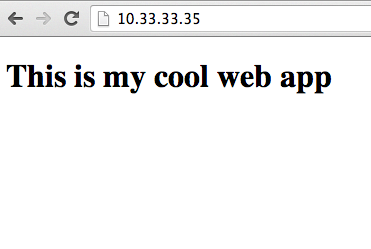
\includegraphics[width=0.6\textwidth]{my_cool_app_index}}
  \caption{Our cool app}
  \label{fig:my_cool_app_index}
\end{figure}